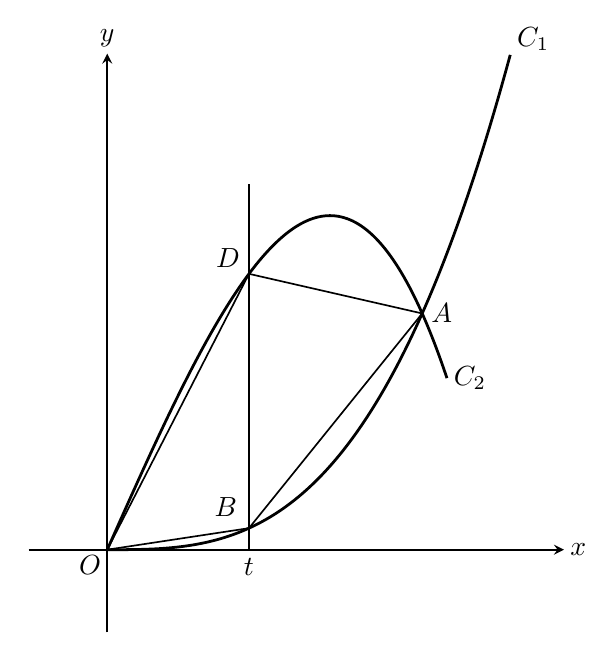
\begin{tikzpicture}[x=4cm,y=3cm,line width=.6pt,>=stealth]
\draw[->] (-0.25,0)--(1.45,0) node[right,inner sep=0pt,xshift=2pt] {$x$};
\draw[->] (0,-0.35)--(0,2.1) node[above,inner sep=0pt,yshift=2pt] {$y$};
\node[below left,inner sep=0pt,xshift=-2pt,yshift=-2pt] at (0,0) {$O$};
\draw[line width=1pt,domain=0:1.28,samples=100] plot (\x,{\x*\x*\x}) node[above right,inner sep=0pt,xshift=2pt,yshift=1pt] {$C_{1}$};
\draw[line width=1pt,domain=0:1.08,samples=120] plot (\x,{-2*\x*\x*\x+3*\x}) node[right,inner sep=0pt,xshift=2pt] {$C_{2}$};
\draw (0.45,0)--(0.45,1.55);
\draw (0,0)--(0.45,0.091125)--(1,1)--(0.45,1.16775)--cycle;
\node[right,inner sep=0pt,xshift=3pt] at (1,1) {$A$};
\node[above left,inner sep=0pt,xshift=-4pt,yshift=4pt] at (0.45,0.091125) {$B$};
\node[above left,inner sep=0pt,xshift=-3pt,yshift=2pt] at (0.45,1.16775) {$D$};
\node[below,inner sep=0pt,yshift=-3pt] at (0.45,0) {$t$};
\end{tikzpicture}
